\section{LTE \formelbuch{3-22}}
    Anforderungen an LTE (Long Term Evolution)
	\begin{liste}
        \item Packet-switched
        \item Round-trip time $< 30$ms
        \item Access time $< 300$ms
        \item Peak rates of 50Mbps for Uplink and 100Mbps for Downlink (in 1st phase)
        \item Flexible Frequenzzuweisung (1.25/2.5, 5, 10, 15, 20MHz)
		\item Nur IP-Services (Ausnahme ist SMS, das weiter mit Signalisierungsmeldungen funktioniert.)
    \end{liste}

\subsection{Downlink}
	LTE verwendet als Zugriffsverfahren im Downlink OFDMA im Gegensatz zu GSM und UMTS.

	\begin{minipage}{9cm}        
        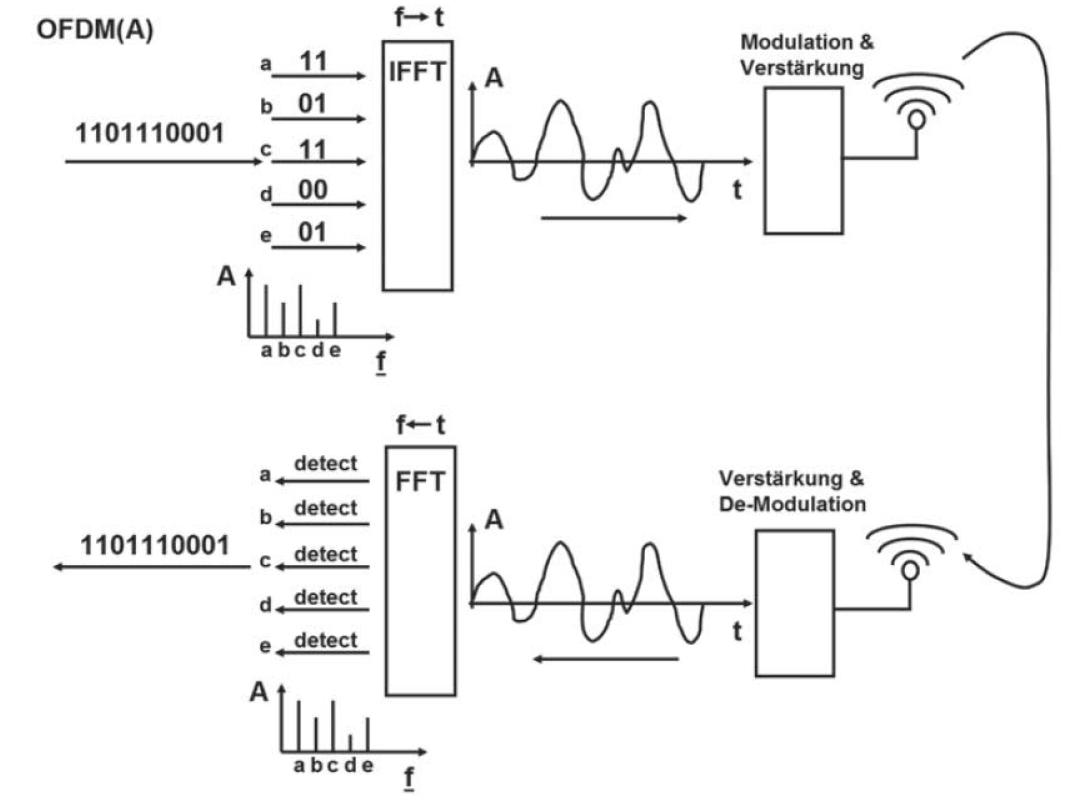
\includegraphics[width=9cm]{./bilder/systems-lte-ofdma.png} \\
        Das obige Bild zeigt, wie die einzelnen Trägersignale bei den verschiedenen Frequenzen mit QPSK moduliert werden.
    \end{minipage}
	\begin{minipage}{0.5cm}        
        \quad
    \end{minipage}
    \begin{minipage}{6.5cm}
		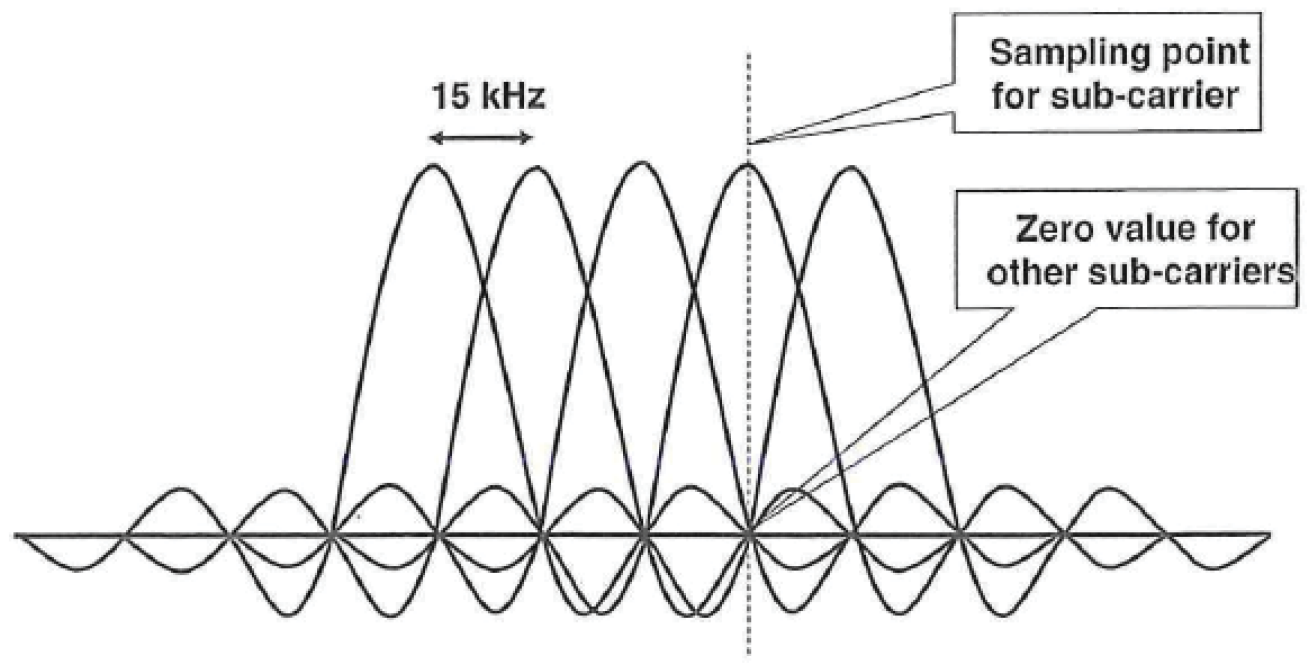
\includegraphics[width=6.5cm]{./bilder/systems-lte-qpsk.png} \\
		Der Trägerabstand beträgt 15kHz, womit eine Nutzsymboldauer von $1/15\text{kHz}=66.7\mu$s resultiert.
	\end{minipage}
	
	
	
